% Options for packages loaded elsewhere
\PassOptionsToPackage{unicode}{hyperref}
\PassOptionsToPackage{hyphens}{url}
%
\documentclass[
]{article}
\usepackage{amsmath,amssymb}
\usepackage{lmodern}
\usepackage{ifxetex,ifluatex}
\ifnum 0\ifxetex 1\fi\ifluatex 1\fi=0 % if pdftex
  \usepackage[T1]{fontenc}
  \usepackage[utf8]{inputenc}
  \usepackage{textcomp} % provide euro and other symbols
\else % if luatex or xetex
  \usepackage{unicode-math}
  \defaultfontfeatures{Scale=MatchLowercase}
  \defaultfontfeatures[\rmfamily]{Ligatures=TeX,Scale=1}
\fi
% Use upquote if available, for straight quotes in verbatim environments
\IfFileExists{upquote.sty}{\usepackage{upquote}}{}
\IfFileExists{microtype.sty}{% use microtype if available
  \usepackage[]{microtype}
  \UseMicrotypeSet[protrusion]{basicmath} % disable protrusion for tt fonts
}{}
\makeatletter
\@ifundefined{KOMAClassName}{% if non-KOMA class
  \IfFileExists{parskip.sty}{%
    \usepackage{parskip}
  }{% else
    \setlength{\parindent}{0pt}
    \setlength{\parskip}{6pt plus 2pt minus 1pt}}
}{% if KOMA class
  \KOMAoptions{parskip=half}}
\makeatother
\usepackage{xcolor}
\IfFileExists{xurl.sty}{\usepackage{xurl}}{} % add URL line breaks if available
\IfFileExists{bookmark.sty}{\usepackage{bookmark}}{\usepackage{hyperref}}
\hypersetup{
  pdftitle={MATH 3080 Lab Project 4},
  pdfauthor={Harrison Webb},
  hidelinks,
  pdfcreator={LaTeX via pandoc}}
\urlstyle{same} % disable monospaced font for URLs
\usepackage[margin=1in]{geometry}
\usepackage{color}
\usepackage{fancyvrb}
\newcommand{\VerbBar}{|}
\newcommand{\VERB}{\Verb[commandchars=\\\{\}]}
\DefineVerbatimEnvironment{Highlighting}{Verbatim}{commandchars=\\\{\}}
% Add ',fontsize=\small' for more characters per line
\usepackage{framed}
\definecolor{shadecolor}{RGB}{248,248,248}
\newenvironment{Shaded}{\begin{snugshade}}{\end{snugshade}}
\newcommand{\AlertTok}[1]{\textcolor[rgb]{0.94,0.16,0.16}{#1}}
\newcommand{\AnnotationTok}[1]{\textcolor[rgb]{0.56,0.35,0.01}{\textbf{\textit{#1}}}}
\newcommand{\AttributeTok}[1]{\textcolor[rgb]{0.77,0.63,0.00}{#1}}
\newcommand{\BaseNTok}[1]{\textcolor[rgb]{0.00,0.00,0.81}{#1}}
\newcommand{\BuiltInTok}[1]{#1}
\newcommand{\CharTok}[1]{\textcolor[rgb]{0.31,0.60,0.02}{#1}}
\newcommand{\CommentTok}[1]{\textcolor[rgb]{0.56,0.35,0.01}{\textit{#1}}}
\newcommand{\CommentVarTok}[1]{\textcolor[rgb]{0.56,0.35,0.01}{\textbf{\textit{#1}}}}
\newcommand{\ConstantTok}[1]{\textcolor[rgb]{0.00,0.00,0.00}{#1}}
\newcommand{\ControlFlowTok}[1]{\textcolor[rgb]{0.13,0.29,0.53}{\textbf{#1}}}
\newcommand{\DataTypeTok}[1]{\textcolor[rgb]{0.13,0.29,0.53}{#1}}
\newcommand{\DecValTok}[1]{\textcolor[rgb]{0.00,0.00,0.81}{#1}}
\newcommand{\DocumentationTok}[1]{\textcolor[rgb]{0.56,0.35,0.01}{\textbf{\textit{#1}}}}
\newcommand{\ErrorTok}[1]{\textcolor[rgb]{0.64,0.00,0.00}{\textbf{#1}}}
\newcommand{\ExtensionTok}[1]{#1}
\newcommand{\FloatTok}[1]{\textcolor[rgb]{0.00,0.00,0.81}{#1}}
\newcommand{\FunctionTok}[1]{\textcolor[rgb]{0.00,0.00,0.00}{#1}}
\newcommand{\ImportTok}[1]{#1}
\newcommand{\InformationTok}[1]{\textcolor[rgb]{0.56,0.35,0.01}{\textbf{\textit{#1}}}}
\newcommand{\KeywordTok}[1]{\textcolor[rgb]{0.13,0.29,0.53}{\textbf{#1}}}
\newcommand{\NormalTok}[1]{#1}
\newcommand{\OperatorTok}[1]{\textcolor[rgb]{0.81,0.36,0.00}{\textbf{#1}}}
\newcommand{\OtherTok}[1]{\textcolor[rgb]{0.56,0.35,0.01}{#1}}
\newcommand{\PreprocessorTok}[1]{\textcolor[rgb]{0.56,0.35,0.01}{\textit{#1}}}
\newcommand{\RegionMarkerTok}[1]{#1}
\newcommand{\SpecialCharTok}[1]{\textcolor[rgb]{0.00,0.00,0.00}{#1}}
\newcommand{\SpecialStringTok}[1]{\textcolor[rgb]{0.31,0.60,0.02}{#1}}
\newcommand{\StringTok}[1]{\textcolor[rgb]{0.31,0.60,0.02}{#1}}
\newcommand{\VariableTok}[1]{\textcolor[rgb]{0.00,0.00,0.00}{#1}}
\newcommand{\VerbatimStringTok}[1]{\textcolor[rgb]{0.31,0.60,0.02}{#1}}
\newcommand{\WarningTok}[1]{\textcolor[rgb]{0.56,0.35,0.01}{\textbf{\textit{#1}}}}
\usepackage{graphicx}
\makeatletter
\def\maxwidth{\ifdim\Gin@nat@width>\linewidth\linewidth\else\Gin@nat@width\fi}
\def\maxheight{\ifdim\Gin@nat@height>\textheight\textheight\else\Gin@nat@height\fi}
\makeatother
% Scale images if necessary, so that they will not overflow the page
% margins by default, and it is still possible to overwrite the defaults
% using explicit options in \includegraphics[width, height, ...]{}
\setkeys{Gin}{width=\maxwidth,height=\maxheight,keepaspectratio}
% Set default figure placement to htbp
\makeatletter
\def\fps@figure{htbp}
\makeatother
\setlength{\emergencystretch}{3em} % prevent overfull lines
\providecommand{\tightlist}{%
  \setlength{\itemsep}{0pt}\setlength{\parskip}{0pt}}
\setcounter{secnumdepth}{-\maxdimen} % remove section numbering
\ifluatex
  \usepackage{selnolig}  % disable illegal ligatures
\fi

\title{MATH 3080 Lab Project 4}
\author{Harrison Webb}
\date{2/3/2022}

\begin{document}
\maketitle

{
\setcounter{tocdepth}{2}
\tableofcontents
}
\hypertarget{problem-1}{%
\section{Problem 1}\label{problem-1}}

\emph{The \texttt{cats} data set (\textbf{MASS}) contains the heart and
body weight of a sample of male and female cats. Use the data set to
estimate a 95\% prediction interval for the body weight of a male cat.
Assume that the body weight of cats is Normally distributed.}

\hypertarget{solution}{%
\paragraph{Solution}\label{solution}}

First, lets look at a boxplot of cat weights by sex, just to get an idea
of the data we are working with.

\begin{Shaded}
\begin{Highlighting}[]
\FunctionTok{boxplot}\NormalTok{(Bwt}\SpecialCharTok{\textasciitilde{}}\NormalTok{Sex, }\AttributeTok{data =}\NormalTok{ cats, }\AttributeTok{col =} \FunctionTok{c}\NormalTok{(}\StringTok{"\#ce2d54"}\NormalTok{, }\StringTok{"\#44135c"}\NormalTok{))}
\end{Highlighting}
\end{Shaded}

\begin{center}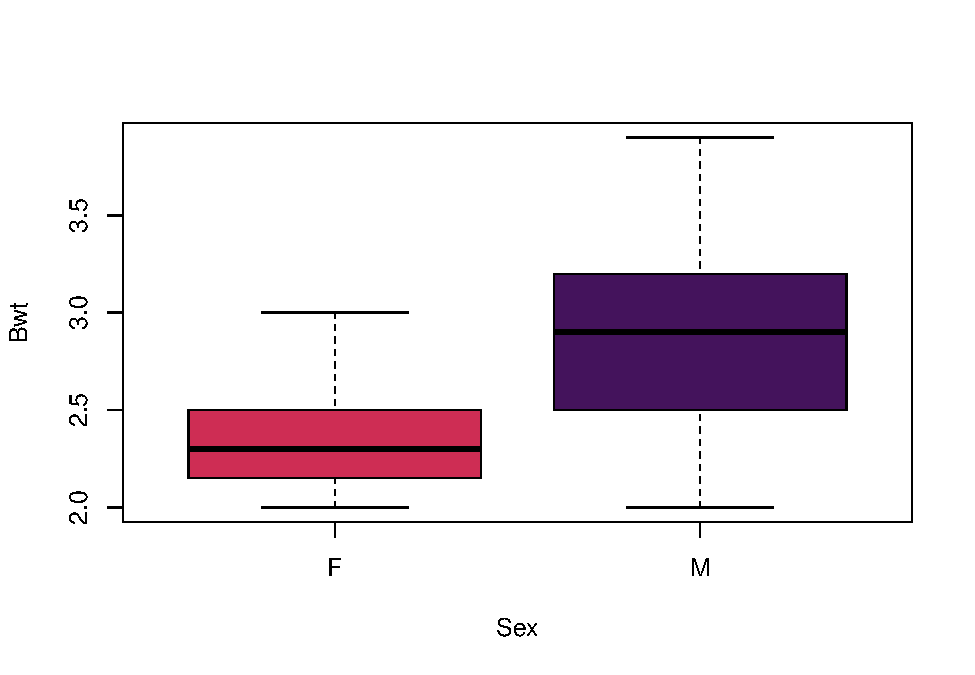
\includegraphics[width=0.75\linewidth]{3080Project4_StatisticalIntervals_files/figure-latex/unnamed-chunk-2-1} \end{center}

Here we see that the weight of male cats is roughly centered around 2.8
or so, and that the values range from roughly 2 to 3.8.

Now we can set up the prediction interval to predict the weight of a
``new'' male cat.

\begin{Shaded}
\begin{Highlighting}[]
\NormalTok{pi\_norm }\OtherTok{\textless{}{-}} \ControlFlowTok{function}\NormalTok{(x, }\AttributeTok{conf.level =} \FloatTok{0.95}\NormalTok{, }\AttributeTok{alternative =} \StringTok{"two.sided"}\NormalTok{) \{}
\NormalTok{  alpha }\OtherTok{\textless{}{-}} \DecValTok{1} \SpecialCharTok{{-}}\NormalTok{ conf.level}
\NormalTok{  n }\OtherTok{\textless{}{-}} \FunctionTok{length}\NormalTok{(x)}
\NormalTok{  xbar }\OtherTok{\textless{}{-}} \FunctionTok{mean}\NormalTok{(x)}
\NormalTok{  err }\OtherTok{\textless{}{-}} \FunctionTok{sd}\NormalTok{(x) }\SpecialCharTok{*} \FunctionTok{sqrt}\NormalTok{(}\DecValTok{1} \SpecialCharTok{+} \DecValTok{1} \SpecialCharTok{/}\NormalTok{ n)}
\NormalTok{  crit }\OtherTok{\textless{}{-}} \ControlFlowTok{switch}\NormalTok{(alternative,}
                 \StringTok{"two.sided"} \OtherTok{=} \FunctionTok{qt}\NormalTok{(alpha }\SpecialCharTok{/} \DecValTok{2}\NormalTok{, }\AttributeTok{df =}\NormalTok{ n }\SpecialCharTok{{-}} \DecValTok{1}\NormalTok{, }\AttributeTok{lower.tail =} \ConstantTok{FALSE}\NormalTok{),}
                 \StringTok{"less"} \OtherTok{=} \SpecialCharTok{{-}}\FunctionTok{qt}\NormalTok{(alpha, }\AttributeTok{df =}\NormalTok{ n }\SpecialCharTok{{-}} \DecValTok{1}\NormalTok{, }\AttributeTok{lower.tail =} \ConstantTok{FALSE}\NormalTok{),}
                 \StringTok{"greater"} \OtherTok{=} \FunctionTok{qt}\NormalTok{(alpha, }\AttributeTok{df =}\NormalTok{ n }\SpecialCharTok{{-}} \DecValTok{1}\NormalTok{, }\AttributeTok{lower.tail =} \ConstantTok{FALSE}\NormalTok{),}
                 \CommentTok{\# Below is the "default" switch, triggered if none of the above}
                 \FunctionTok{stop}\NormalTok{(}\StringTok{"alternative must be one of two.sided, less, greater"}\NormalTok{))}
\NormalTok{  interval }\OtherTok{\textless{}{-}} \ControlFlowTok{switch}\NormalTok{(alternative,}
                     \StringTok{"two.sided"} \OtherTok{=} \FunctionTok{c}\NormalTok{(xbar }\SpecialCharTok{{-}}\NormalTok{ crit }\SpecialCharTok{*}\NormalTok{ err, xbar }\SpecialCharTok{+}\NormalTok{ crit }\SpecialCharTok{*}\NormalTok{ err),}
                     \StringTok{"less"} \OtherTok{=} \FunctionTok{c}\NormalTok{(xbar }\SpecialCharTok{+}\NormalTok{ crit }\SpecialCharTok{*}\NormalTok{ err, }\ConstantTok{Inf}\NormalTok{),}
                     \StringTok{"greater"} \OtherTok{=} \FunctionTok{c}\NormalTok{(}\SpecialCharTok{{-}}\ConstantTok{Inf}\NormalTok{, xbar }\SpecialCharTok{+}\NormalTok{ crit }\SpecialCharTok{*}\NormalTok{ err),}
                     \FunctionTok{stop}\NormalTok{(}\StringTok{"How did I get here?"}\NormalTok{))}
  \FunctionTok{attr}\NormalTok{(interval, }\StringTok{"conf.level"}\NormalTok{) }\OtherTok{\textless{}{-}}\NormalTok{ conf.level}
\NormalTok{  interval}
\NormalTok{\}}

\NormalTok{data }\OtherTok{=} \FunctionTok{subset}\NormalTok{(cats, }\AttributeTok{subset =}\NormalTok{ Sex }\SpecialCharTok{==} \StringTok{\textquotesingle{}M\textquotesingle{}}\NormalTok{)}\SpecialCharTok{$}\NormalTok{Bwt}

\FunctionTok{pi\_norm}\NormalTok{(data)}
\end{Highlighting}
\end{Shaded}

\begin{verbatim}
## [1] 1.96728 3.83272
## attr(,"conf.level")
## [1] 0.95
\end{verbatim}

\hypertarget{problem-2}{%
\section{Problem 2}\label{problem-2}}

\emph{The data set \texttt{SP500} (\textbf{MASS}) contains the returns
of the S\&P 500 stock index for the 1990s; that is, it's the ratio of
the change of the index's price divided by the preceding day price. In
principle, when predicting the direction of the stock market with the
intention of buying stock, we are willing to be wrong in one direction
but not another; we are okay with predicting the market grows too little
and be pleasantly surprised than to predict the market grows more than
it actually does. So compute a 99\% lower prediction bound, assuming
that stock returns are Normally distributed. (You should not trust this
number. First the Normality assumption, despite being assumed a lot in
finance, is not true. Second, stock returns are} not \emph{an
independent and identically distributed sample.)}

\hypertarget{solution-1}{%
\paragraph{Solution}\label{solution-1}}

\begin{Shaded}
\begin{Highlighting}[]
\CommentTok{\# Your code here}
\end{Highlighting}
\end{Shaded}

\hypertarget{problem-3}{%
\section{Problem 3}\label{problem-3}}

\emph{The data set \texttt{abbey} (\textbf{MASS}) contains
determinations of nickel content (ppm) in a Canadian syenite rock. The
assumption of a Normal distribution clearly is inappropriate for this
data set. Construct a 90\% prediction interval for the next measurement
from the data set. Use a nonparametric procedure.}

\begin{Shaded}
\begin{Highlighting}[]
\CommentTok{\# Your code here}
\end{Highlighting}
\end{Shaded}

\hypertarget{problem-4}{%
\section{Problem 4}\label{problem-4}}

\emph{Use the data from Problem 1 to construct a 95\% tolerance interval
for 99\% of cats' body weight.}

\begin{Shaded}
\begin{Highlighting}[]
\CommentTok{\# Your code here}
\end{Highlighting}
\end{Shaded}

\hypertarget{problem-5}{%
\section{Problem 5}\label{problem-5}}

\emph{The data set \texttt{geyser} (\textbf{MASS}) contains both wait
time between and duration of eruptions of the Old Faithful geyser in
Yellowstone National Park. Use the data set to construct a nonparametric
tolerance interval containing 90\% of geyser eruptions with 99\%
confidence.}

\begin{Shaded}
\begin{Highlighting}[]
\CommentTok{\# Your code here}
\end{Highlighting}
\end{Shaded}

\hypertarget{problem-6}{%
\section{Problem 6}\label{problem-6}}

\emph{The data set \texttt{accdeaths} (\textbf{MASS}) contains a count
of accidental deaths in the United States between 1973 and 1978. What
was the mean count of accidental deaths per month? Use this data set to
construct a statistical interval for the mean number of accidental
deaths over the next five years. (Bonus points if you can compare your
interval to the observed mean over those years and assess how well it
did.)}

\begin{Shaded}
\begin{Highlighting}[]
\CommentTok{\# Your code here}
\end{Highlighting}
\end{Shaded}


\end{document}
